\documentclass[main.tex]{subfiles}
\begin{document}
\begin{enumerate}

\subsection{Section 8}

\item A three-phase 250MVA, 20kV, 60Hz salient pole synchronous machine has parameters Xd = 1.1 pu, Xq = 0.6 pu and Ra~0. The machine delivers 230MW at 0.9 lagging power factor to an infinite busbar. Calculate the excitation voltage and power angle. Draw the phasor diagram. (Hint: use per unit values and give your answers in pu).

\item A wind turbine is to be designed with an electrical power output of 7.0MW. The rated upwind free wind speed is 13 m/s. Determine the length of the rotor blades and the height of the supporting tower in meters and the rotational speed of the rotor in rev/min if the tip-speed ratio whose value as 7.0 determines the maximum Power Coefficient of 0.45. Use the density of air as $\num{1.225}\unit{kg/m^3}$

\item A 450MVA, 20kV, 60-Hz round-rotor synchronous generator has an Inertia constant H = 5s. Displayed on the axes in Figure \ref{fig:24q_a} are Torque/Angle characteristics for various faults occurring on a double circuit transmission line when connected between a synchronous generator and an infinite busbar. Using the Equal Area Criterion, determine the critical switching times for both a $3 \varphi$ fault and a Line to Line fault when the input and torque from the turbine is 1.0 pu as shown in the diagram.

\begin{figure}
\centering\fbox{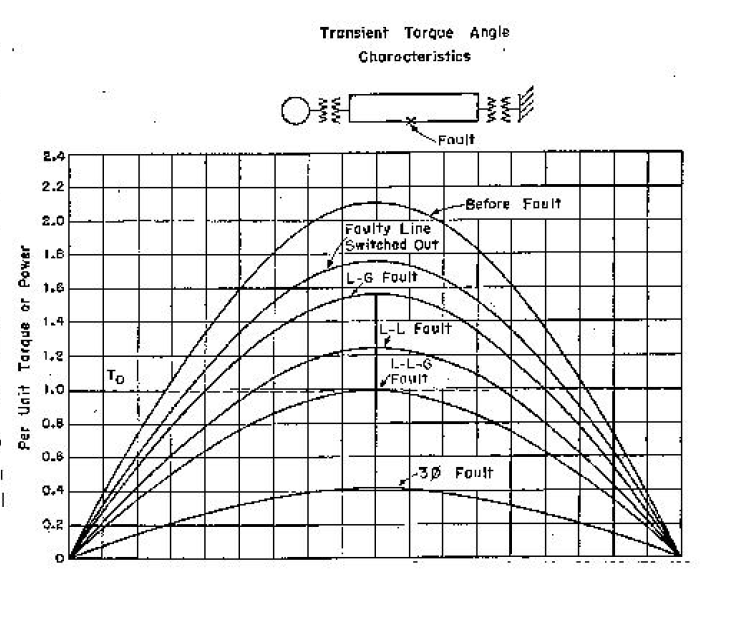
\includegraphics[width=4.0in]{figures/2018s/24q_a.png}}
\caption{Transient Torque Angle}
\label{fig:24q_a}
\end{figure}

\end{enumerate}
\end{document}